\documentclass{article}
\usepackage{graphicx} % Required for inserting images
\usepackage[natbibapa]{apacite}
\usepackage[colorlinks=true,linkcolor=black,citecolor=black,urlcolor=black]{hyperref}
\usepackage{amsmath}


\title{\vspace{-2cm}Assignment 1\\
    The Scientific Discourse}

\author{Tymur Mykhalievskyi\\ 7031100}
\date{\today}


\begin{document}

\maketitle

\section{General Overview}
The original work by \cite{reshef2011} introduces a new metric called MIC. The topic quickly gained popularity and was followed by a number of papers that either criticize the work or try to improve it. In this review we will focus on the critique towards MIC. The main goal of this review is to provide a critical overview of the work by \cite{reshef2011} and to discuss the limitations of MIC. 

\section{Scientific Discourse on MIC}
\label{sec:discourse}
In my opinion, the work by \cite{reshef2011} got a lot of attention because it was the first work that introduced a new metric that is supposed to be general and equitable. But even more importantly, the whole idea of MIC seems rather intuitive, does not involve complicated mathematics and was tested on empirical data. 

The first critique towards MIC we will look at was presented by \cite{simon2014}. The following quote summarizes the main point: 
\begin{quote}
    ``This set of dependencies is by no means exhaustive, however it suggests that MIC has serious power deficiencies, and hence when it is used for large-scale exploratory analysis it will produce too many false positives. The ``equitability'' property of MIC is not very useful, if it has low power.''
\end{quote}

I would agree with the main point of lack of power by \cite{simon2014}. However, while the authors argue MIC yields false positives, the low power of MIC more directly leads to false negatives — i.e., failing to detect true relationships. False positives may still occur under multiple testing without correction.

Further, more thorough critique by \cite{kinney2014} tries to argue that the metric is not as equitable as it is claimed to be. The main problem is that \cite{reshef2011} did not provide a formal definition of equitability, but rather an operationalization. Hence, \cite{kinney2014} suggested a formal definition of equitability that they call ``self-equitability''. While some of the points were definitely valid, such as inconsistency of MIC \citep{kinney2014} (Figure 3), the main point of the paper is that the metric is not ``self-equitable'' enough, which it never claimed to be. 

\sloppy
Hence, there appeared an expected response by \cite{reshef2014}. They pointed out that ``self-equitability'' was not the goal of the original work. Furthermore, \cite{reshef2014} were not satisfied with the comparisons of MIC and another mutual information estimation method by \cite{kinney2014}. Therefore, a more thorough comparison was made. However, the main problem remains, equitability according to \cite{reshef2014} is still not formal and definitely does not align with self-equitability. 

The follow up by \cite{kinney20142} points out exactly the same problem. Equitability by \cite{reshef2014} is still not defined formally, therefore, allowing \cite{reshef2014} to interpret the results in a way that is convenient for them.

Finally, the formal definition according to \cite{reshef2015} was presented, and similar results to their last response were shown \citep{reshef2014}.

\subsection{Contextual Considerations}
It is worth noting that, PNAS is high-profile and benefits from buzzworthy articles. MIC was such a paper. That said, academic journals do not make money like newspapers, and PNAS is run by the National Academy of Sciences. Therefore, it's unlikely that money alone drove the decision of publishing the comments by \cite{kinney2014}. However, money could have contributed to the decision of publishing such comments.

In addition, the work by \cite{simon2014} and \cite{reshef2015} was shared via arXiv. This means that the paper is available as soon as it added as a pre-print, without need to wait for a review. On one hand this allows for a quicker exchange of information. On the other hand, it is a way to bypass the peer-review process. This is a double-edged sword, allowing for a quicker and perhaps more open exchange of information. But also allowing for the publication of papers that are not peer-reviewed, meaning that they are not necessarily correct or of high quality.


\subsubsection*{Conclusion}
To summarize, the discourse around MIC was very well justified in my opinion. Every author is biased to some extent, and therefore, seeing different points of view is crucial, in order to understand the full picture.

One could argue that the original work by \cite{reshef2011} should not have been published in the first place, as it does not provide a formal definition of equitability. However, I would argue that the work was important. The metric is definitely not perfect, but it is a good starting point for further research. 

\section{MIC}
In this section we will critically discuss MIC. The overall idea seems promising on the first glance. MIC is supposed to be the one metric that is general and equitable (according to the definition by \cite{reshef2011}). Reading the work by \cite{reshef2011}, prima facie, MIC completely satisfies these properties. In particular, MIC does not make any assumptions about the underlying function which is supposed to make it generalize very well. However, after reading the concerns presented by \cite{simon2014} and \cite{kinney2014}, a more thorough analysis of MIC had to be conducted.


\subsection{Time Complexity and Grid Resolution}
In my opinion, the main problem of MIC lies in the time complexity of the algorithm. The time complexity of the original algorithm that estimates MIC \citep{reshef2011} is given by
\[
    O(n^{4\cdot\alpha}) = O(n^{2.4}) \text{ for } \alpha = 0.6
\]
Hence, the time complexity is rather high. Furthermore, the slowest runs of MIC are observed on random data \citep{shao2021}. This is problematic because the algorithm is supposed to be used for exploratory data analysis, and most of the dependencies in the exploratory data analysis are random. Therefore, applying original approximate algorithm of MIC
to detect bivariate relationships in high dimensional data would require a lot of computational resources.

In addition, the grid resolution is bounded by $xy < B(n) < n^\alpha$, where alpha is suggested to be $0.6$. Increase in grid resolution leads to an increase in power \citep{cao2021} (Figure 4). At the same time, the increase in grid resolution leads to an increase in time complexity.


\subsection{Geometrical Interpretation of MIC}
The underlying implementation of MIC is based on the idea of partitioning the scatter plot of two variables into a grid. At this point we can spot an important limitation of MIC which also does not align with the equitability property of the metric. Due to the fact that the grid is made of rectangles, some relationships between two variables could work particularly well. For example, consider two functions: step and modular. The choice of functions in this example is only based on the geometrical look of them. if the underlying function is a step function, the grid would capture the relationship very well. However, if we exchange the underlying function to a modular function, the grid would not be able to capture the relationship as well \autoref{fig:step_mod}. This is because the step function would be able to fit into the grid cells very well, while the modular function, not aligned with either axis, would not be able to fit into the grid cells. 

Notice that the step function is assigned with MIC score of 1, while the modular function only achieves a score around 0.7. Furthermore if we inverse x and y to achieve a slightly different scatter plot (bottom plots of \autoref{fig:step_mod}), we would get the same picture. It is worth noting that by no means a thorough comparison is made here. This is only a demonstration of a particular case. However, the effect persists for other values of the parameters. This limitation arises from MIC's reliance on axis-aligned rectangular partitions, which inherently favor functions that are monotonic or step-like along x or y. Therefore, a more rectangular and parallel to the axis function would be able to fit into the grid cells better. Therefore, getting a higher MIC score. 

\begin{figure}
    \centering
    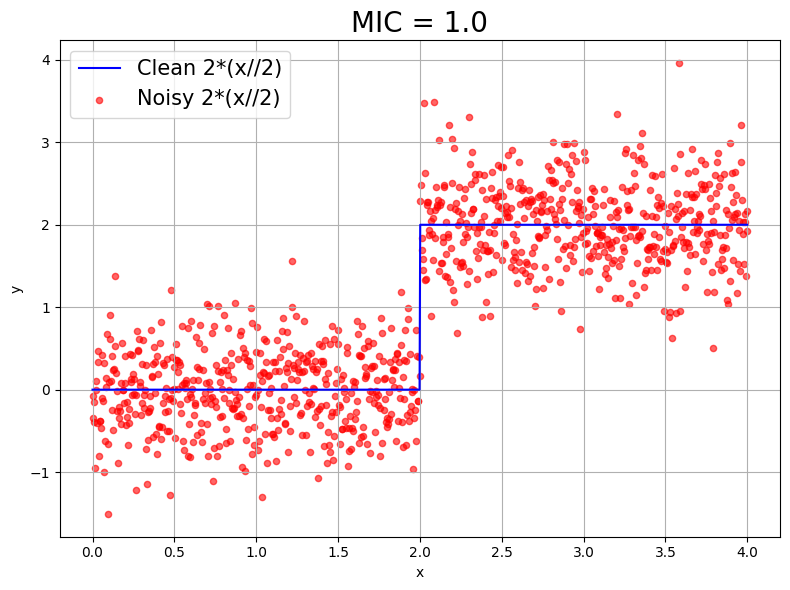
\includegraphics[width=0.47\textwidth]{images/step1.png}
    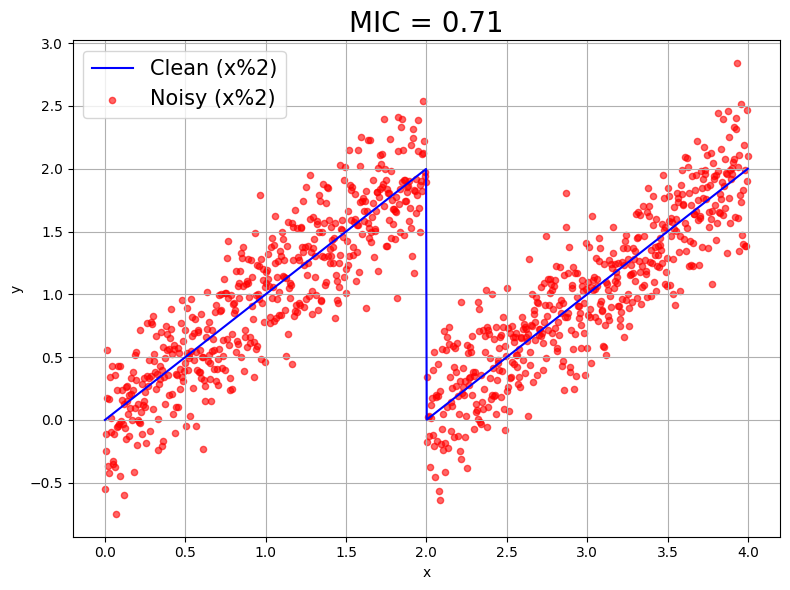
\includegraphics[width=0.47\textwidth]{images/mod1.png}
    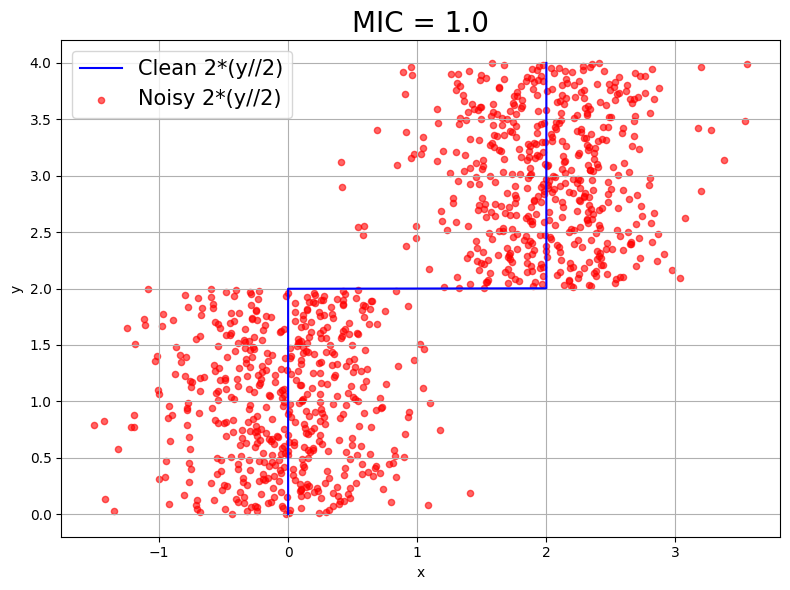
\includegraphics[width=0.47\textwidth]{images/step2.png}
    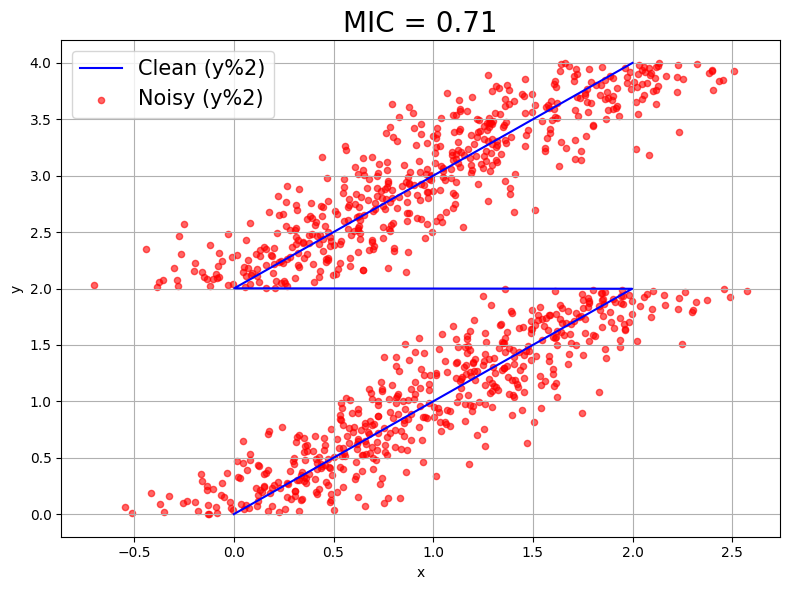
\includegraphics[width=0.47\textwidth]{images/mod2.png}
    \caption{Comparison of the step function and modular function. The left plot shows the step function with its inverse variant on the bottom. While the right plot shows the modular function with its inverse variant. MIC was computed via minepy library \citep{minepy}. Both plots were generated using the exact same parameters: $n = 1000, 1-R^2=0.2, x\in [0, 4)$. The source code is available via GitHub under ``Assignment 1'' \citep{src}.}
    \label{fig:step_mod}
\end{figure}

\section{Equitability}
When analyzing data without strong prior hypotheses, a common goal is to identify a broad range of potentially interesting relationships — regardless of their specific functional form. In such exploratory settings, a desirable property of a dependence measure is equitability. An equitable statistic should assign similar scores to equally noisy relationships, even if the underlying patterns differ (e.g., linear, quadratic, sinusoidal). This would allow researchers to rank associations not by their shape but by how well one variable predicts the other — that is, which is strongly related by the amount of noise in the data.

However, while equitability is a valuable property, it is not sufficient on its own. As \cite{simon2014} emphasized, statistical power — the ability to detect a relationship when one exists — is equally critical. A measure with low power may fail to assign high scores to meaningful but noisy relationships, resulting in false negatives. In practical terms, this means MIC might only highlight obvious, low-noise patterns — which could already be known to the analyst — and miss subtler but potentially more novel findings.


\section{Conclusion}
While MIC is a very interesting metric, it has two main issues: low power and high time complexity. That being said, MIC might be on a more intuitive level than other mutual information estimators, which could enhance the interpretability. However, currently there is no straightforward way to visualize the best grid as it was presented in the original work \citep{reshef2011} (Figure 1). \cite{cao2021} achieved some progress in this task. 

Finally, the broader scientific discourse around MIC, as outlined in \autoref{sec:discourse}, highlights how important it is for novel metrics to be both clearly defined and rigorously evaluated. The debates around equitability, statistical power, and consistency have led to more formal definitions and improved metrics. In this sense, MIC played an important role in advancing the discussion on general-purpose dependence measures — even if it ultimately fell short of its ambitious goals. It serves as a valuable starting point and a reminder that simplicity, interpretability, and rigor must all be carefully balanced in statistical methodology.




\bibliographystyle{apacite}	
\bibliography{references}


\end{document}


